

\chapter{نمودار کلاس طراحی و  نمودار مولفه}
\label{chapter:classDesign}

در ادامه نمودار کلاس‌های طراحی و مولفه‌ها قرار گرفته است.

%\KOMAoptions{paper=a2}
%\recalctypearea
\eject \pdfpagewidth=12in \pdfpageheight=15in

\begin{figure}[ht!]
	\centering
	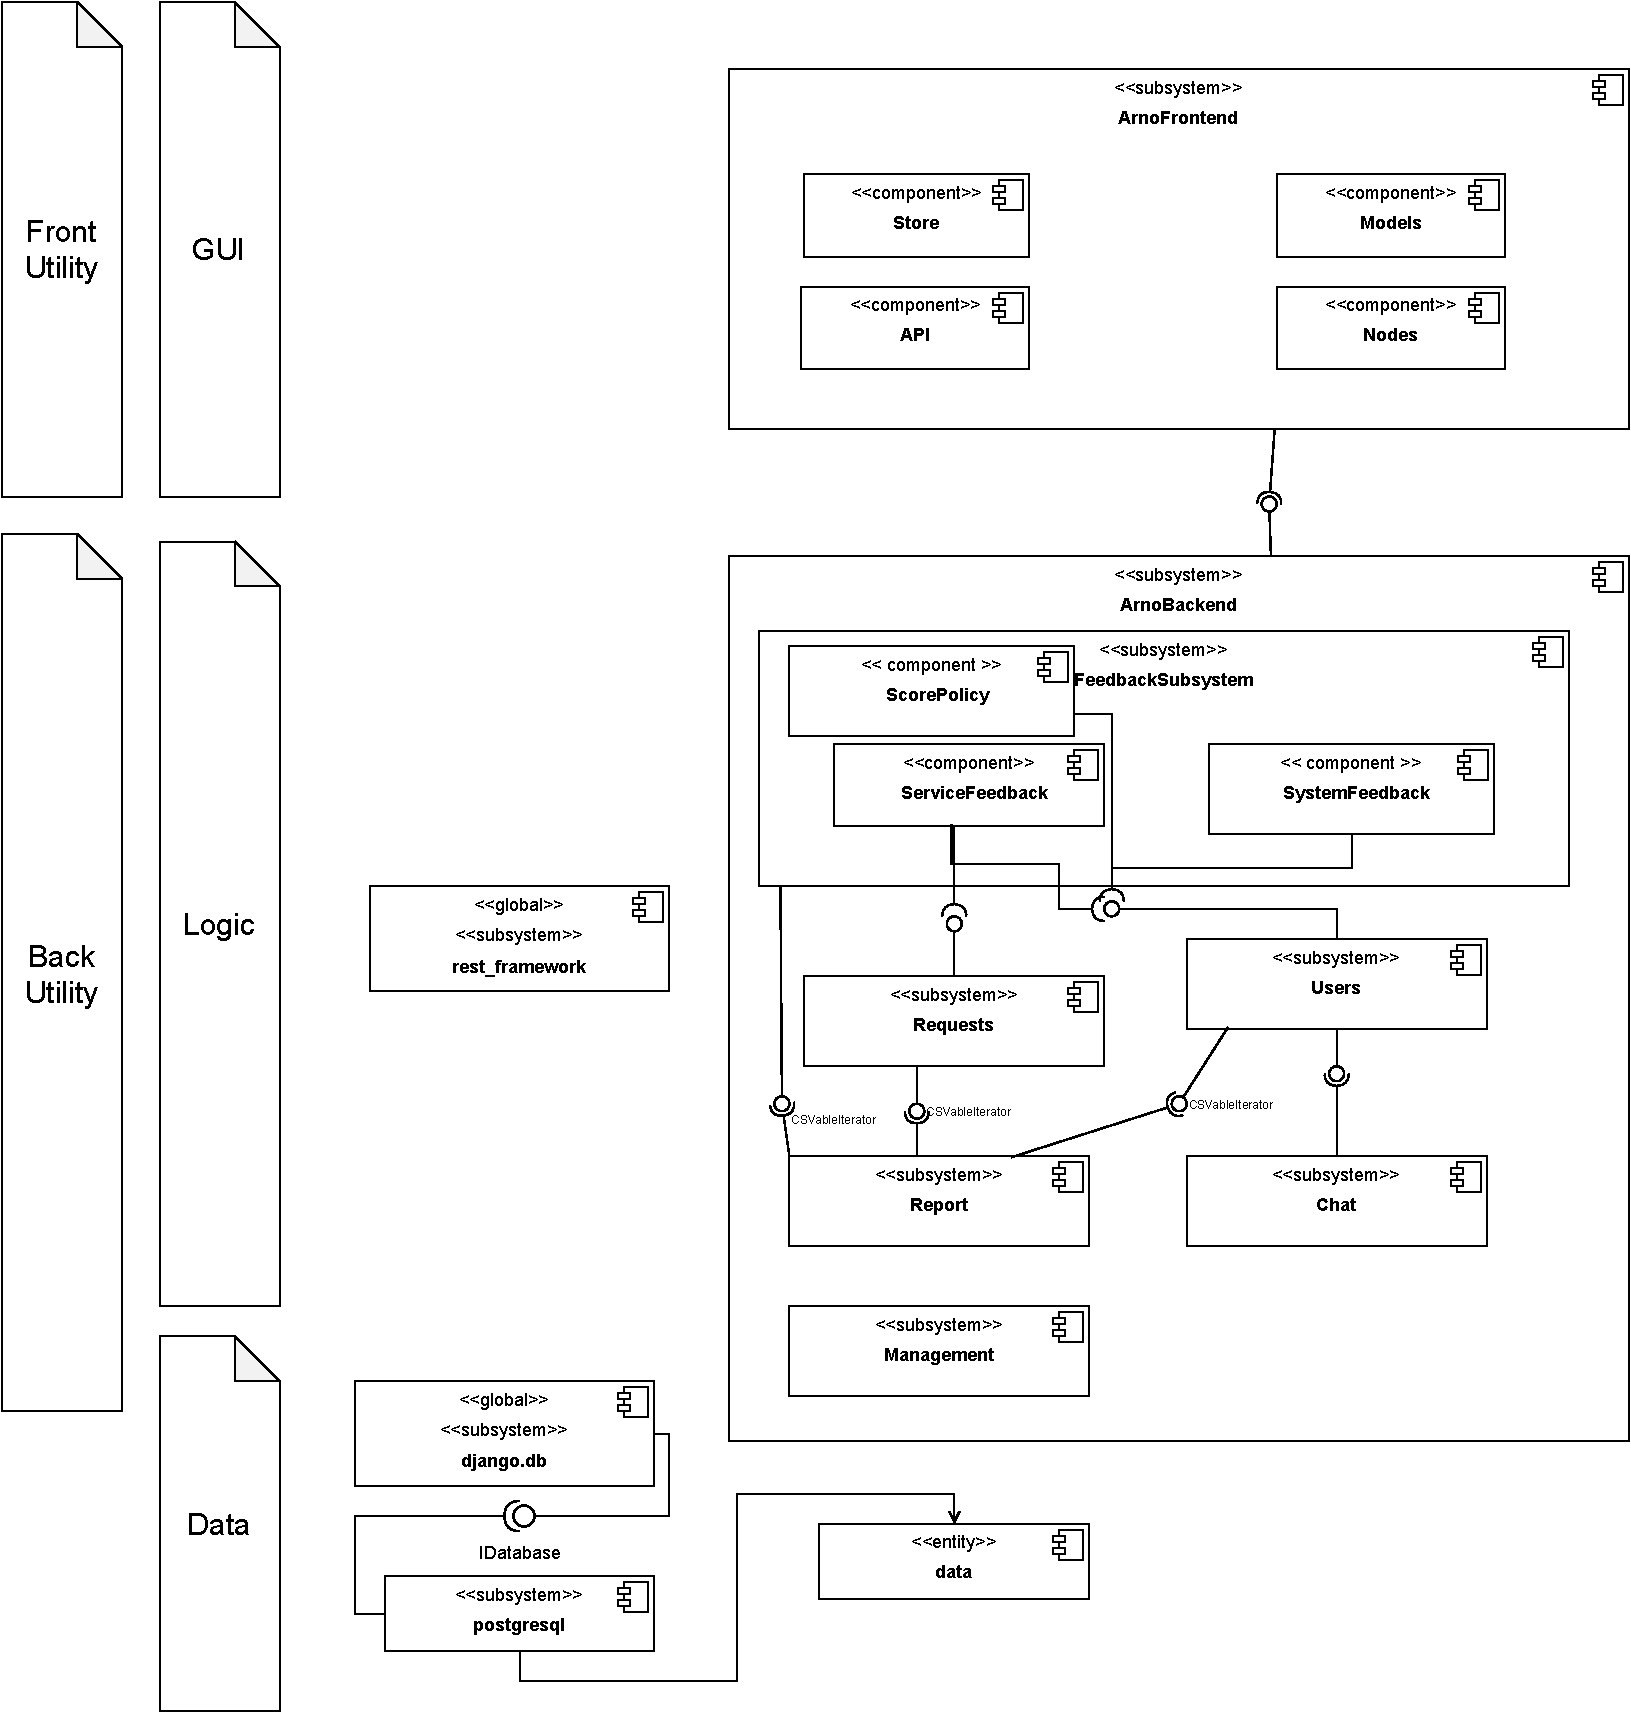
\includegraphics[scale=0.8]{figs/design-class/comps.pdf}
	\caption{مولفه‌ها}
\end{figure}
\FloatBarrier
\newpage

\eject \pdfpagewidth=21in \pdfpageheight=15in

\begin{figure}[ht!]
	\centering
	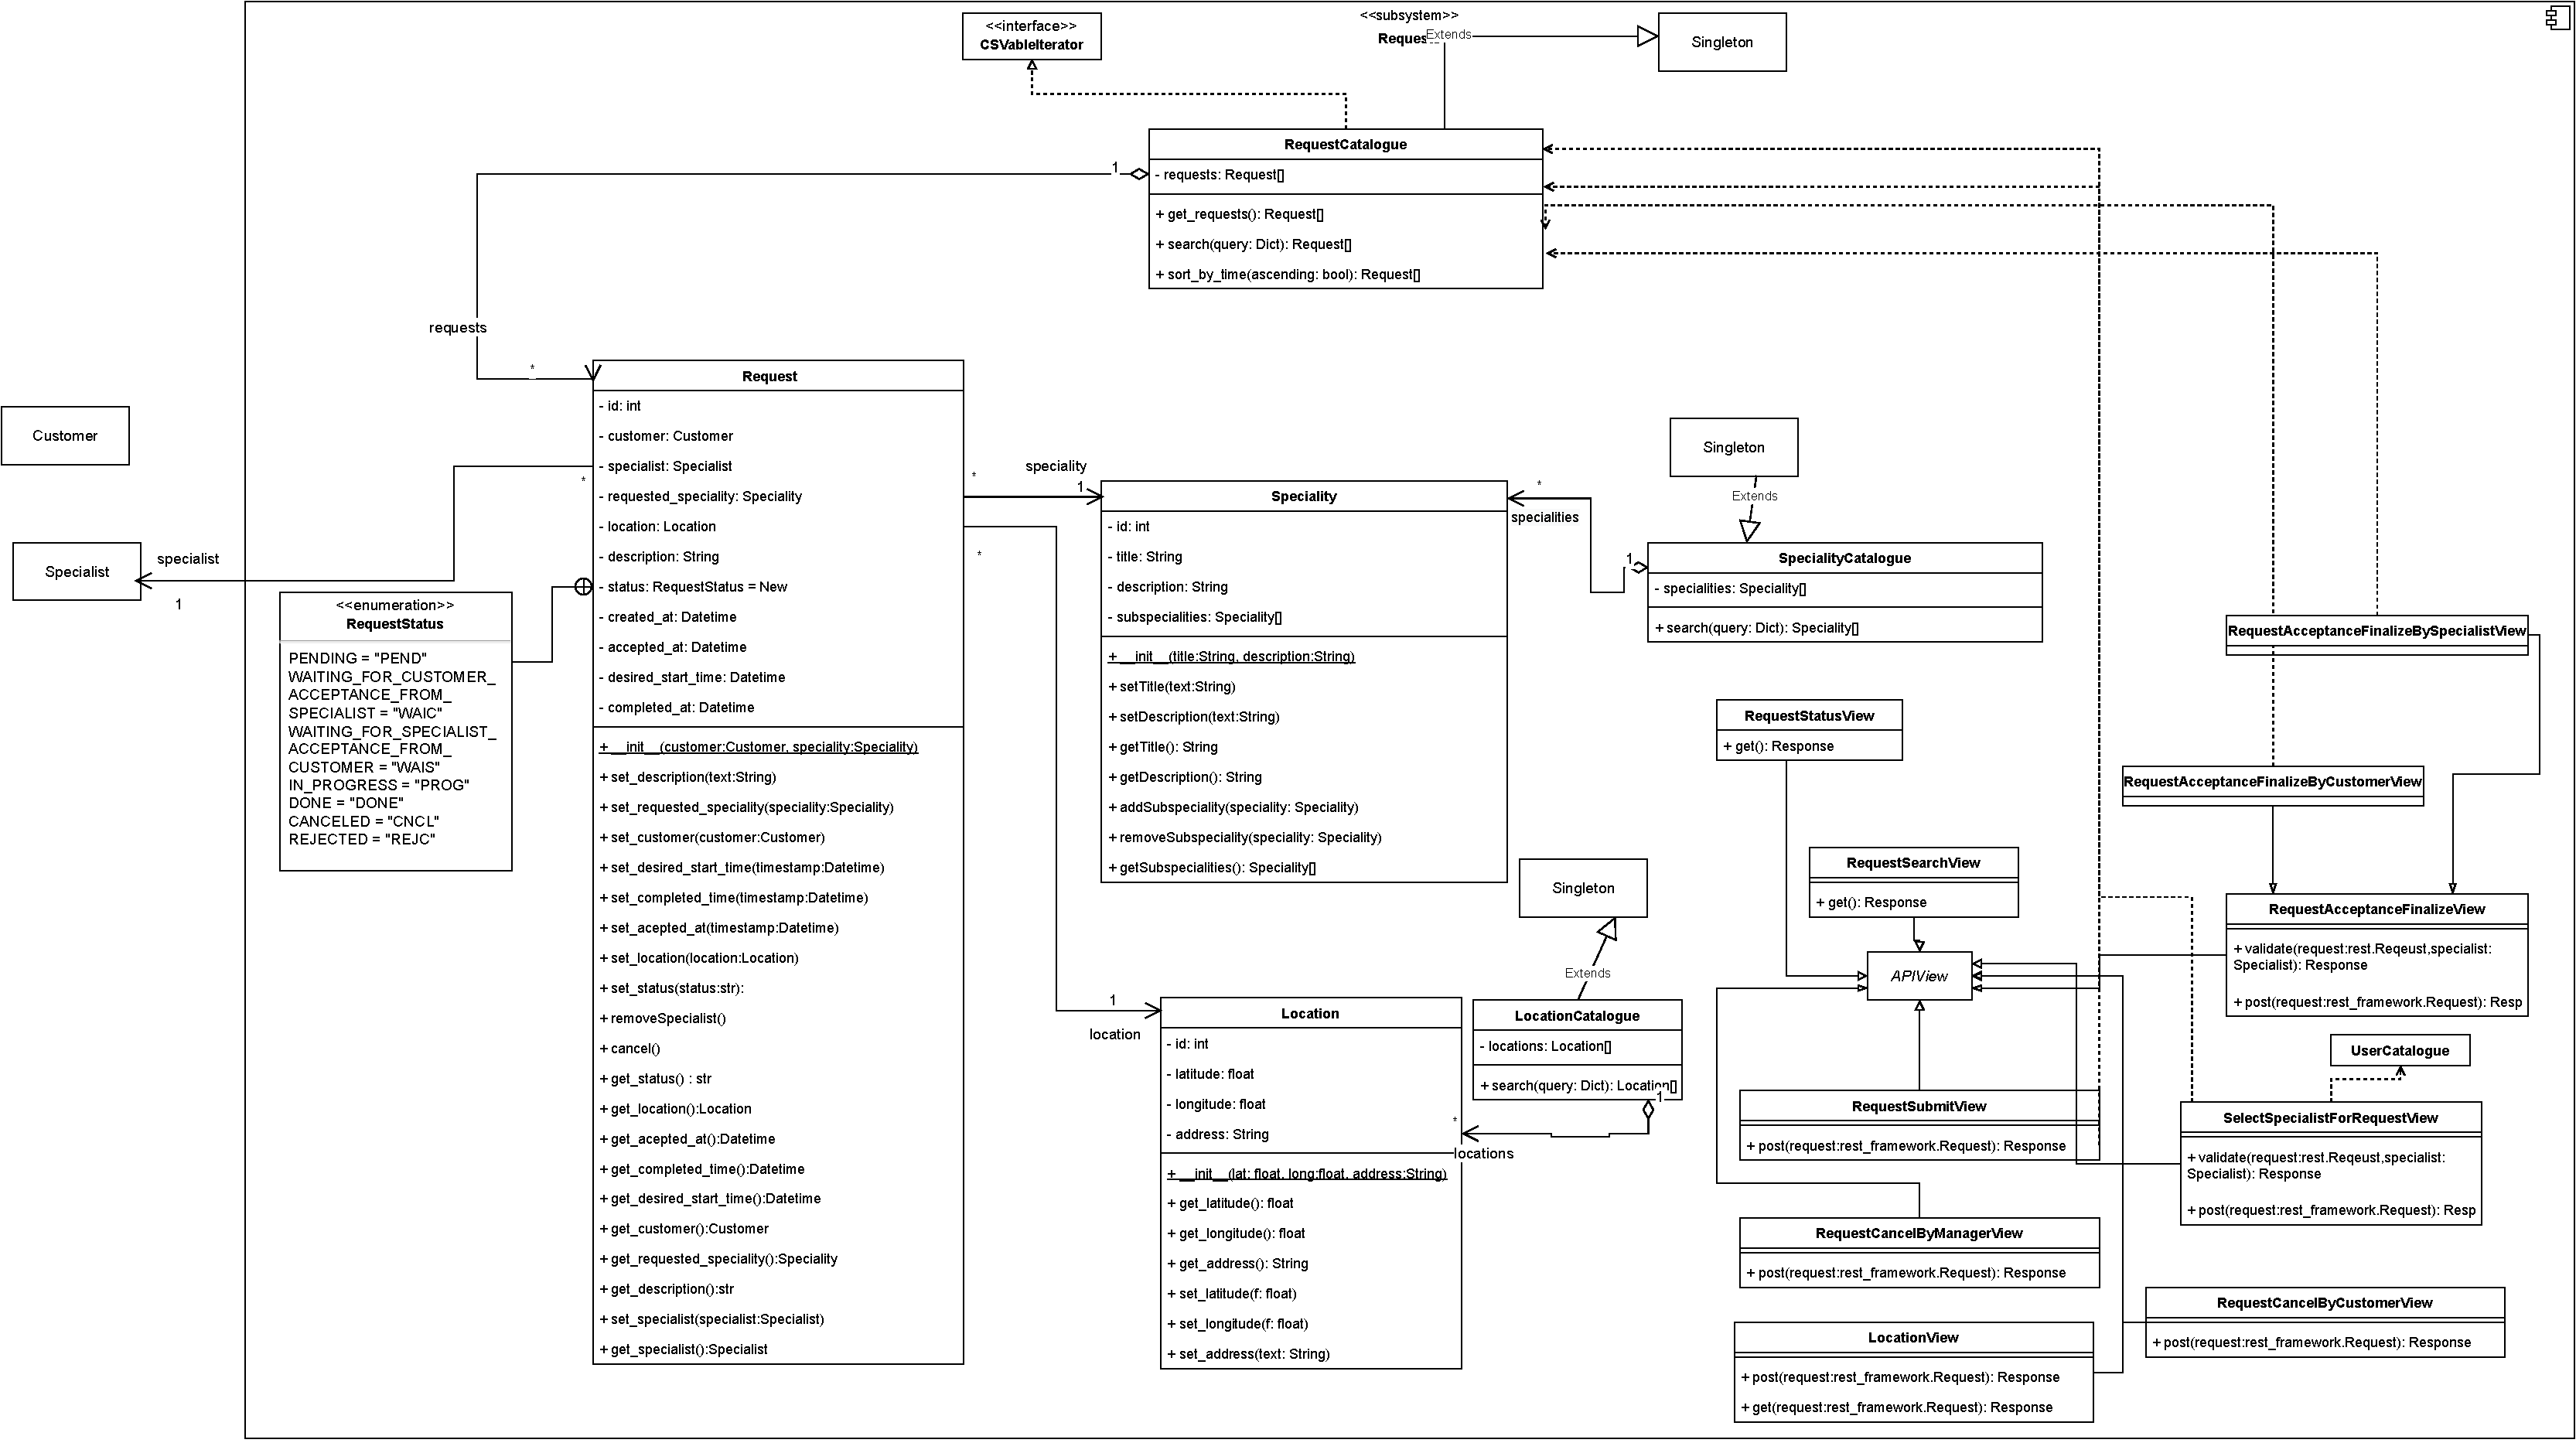
\includegraphics[scale=0.8]{figs/design-class/requests.pdf}
	\caption{کلاس‌های طراحی مولفه درخواست}
\end{figure}
\FloatBarrier
\newpage


\eject \pdfpagewidth=15in \pdfpageheight=18in

\begin{figure}[ht!]
	\centering
	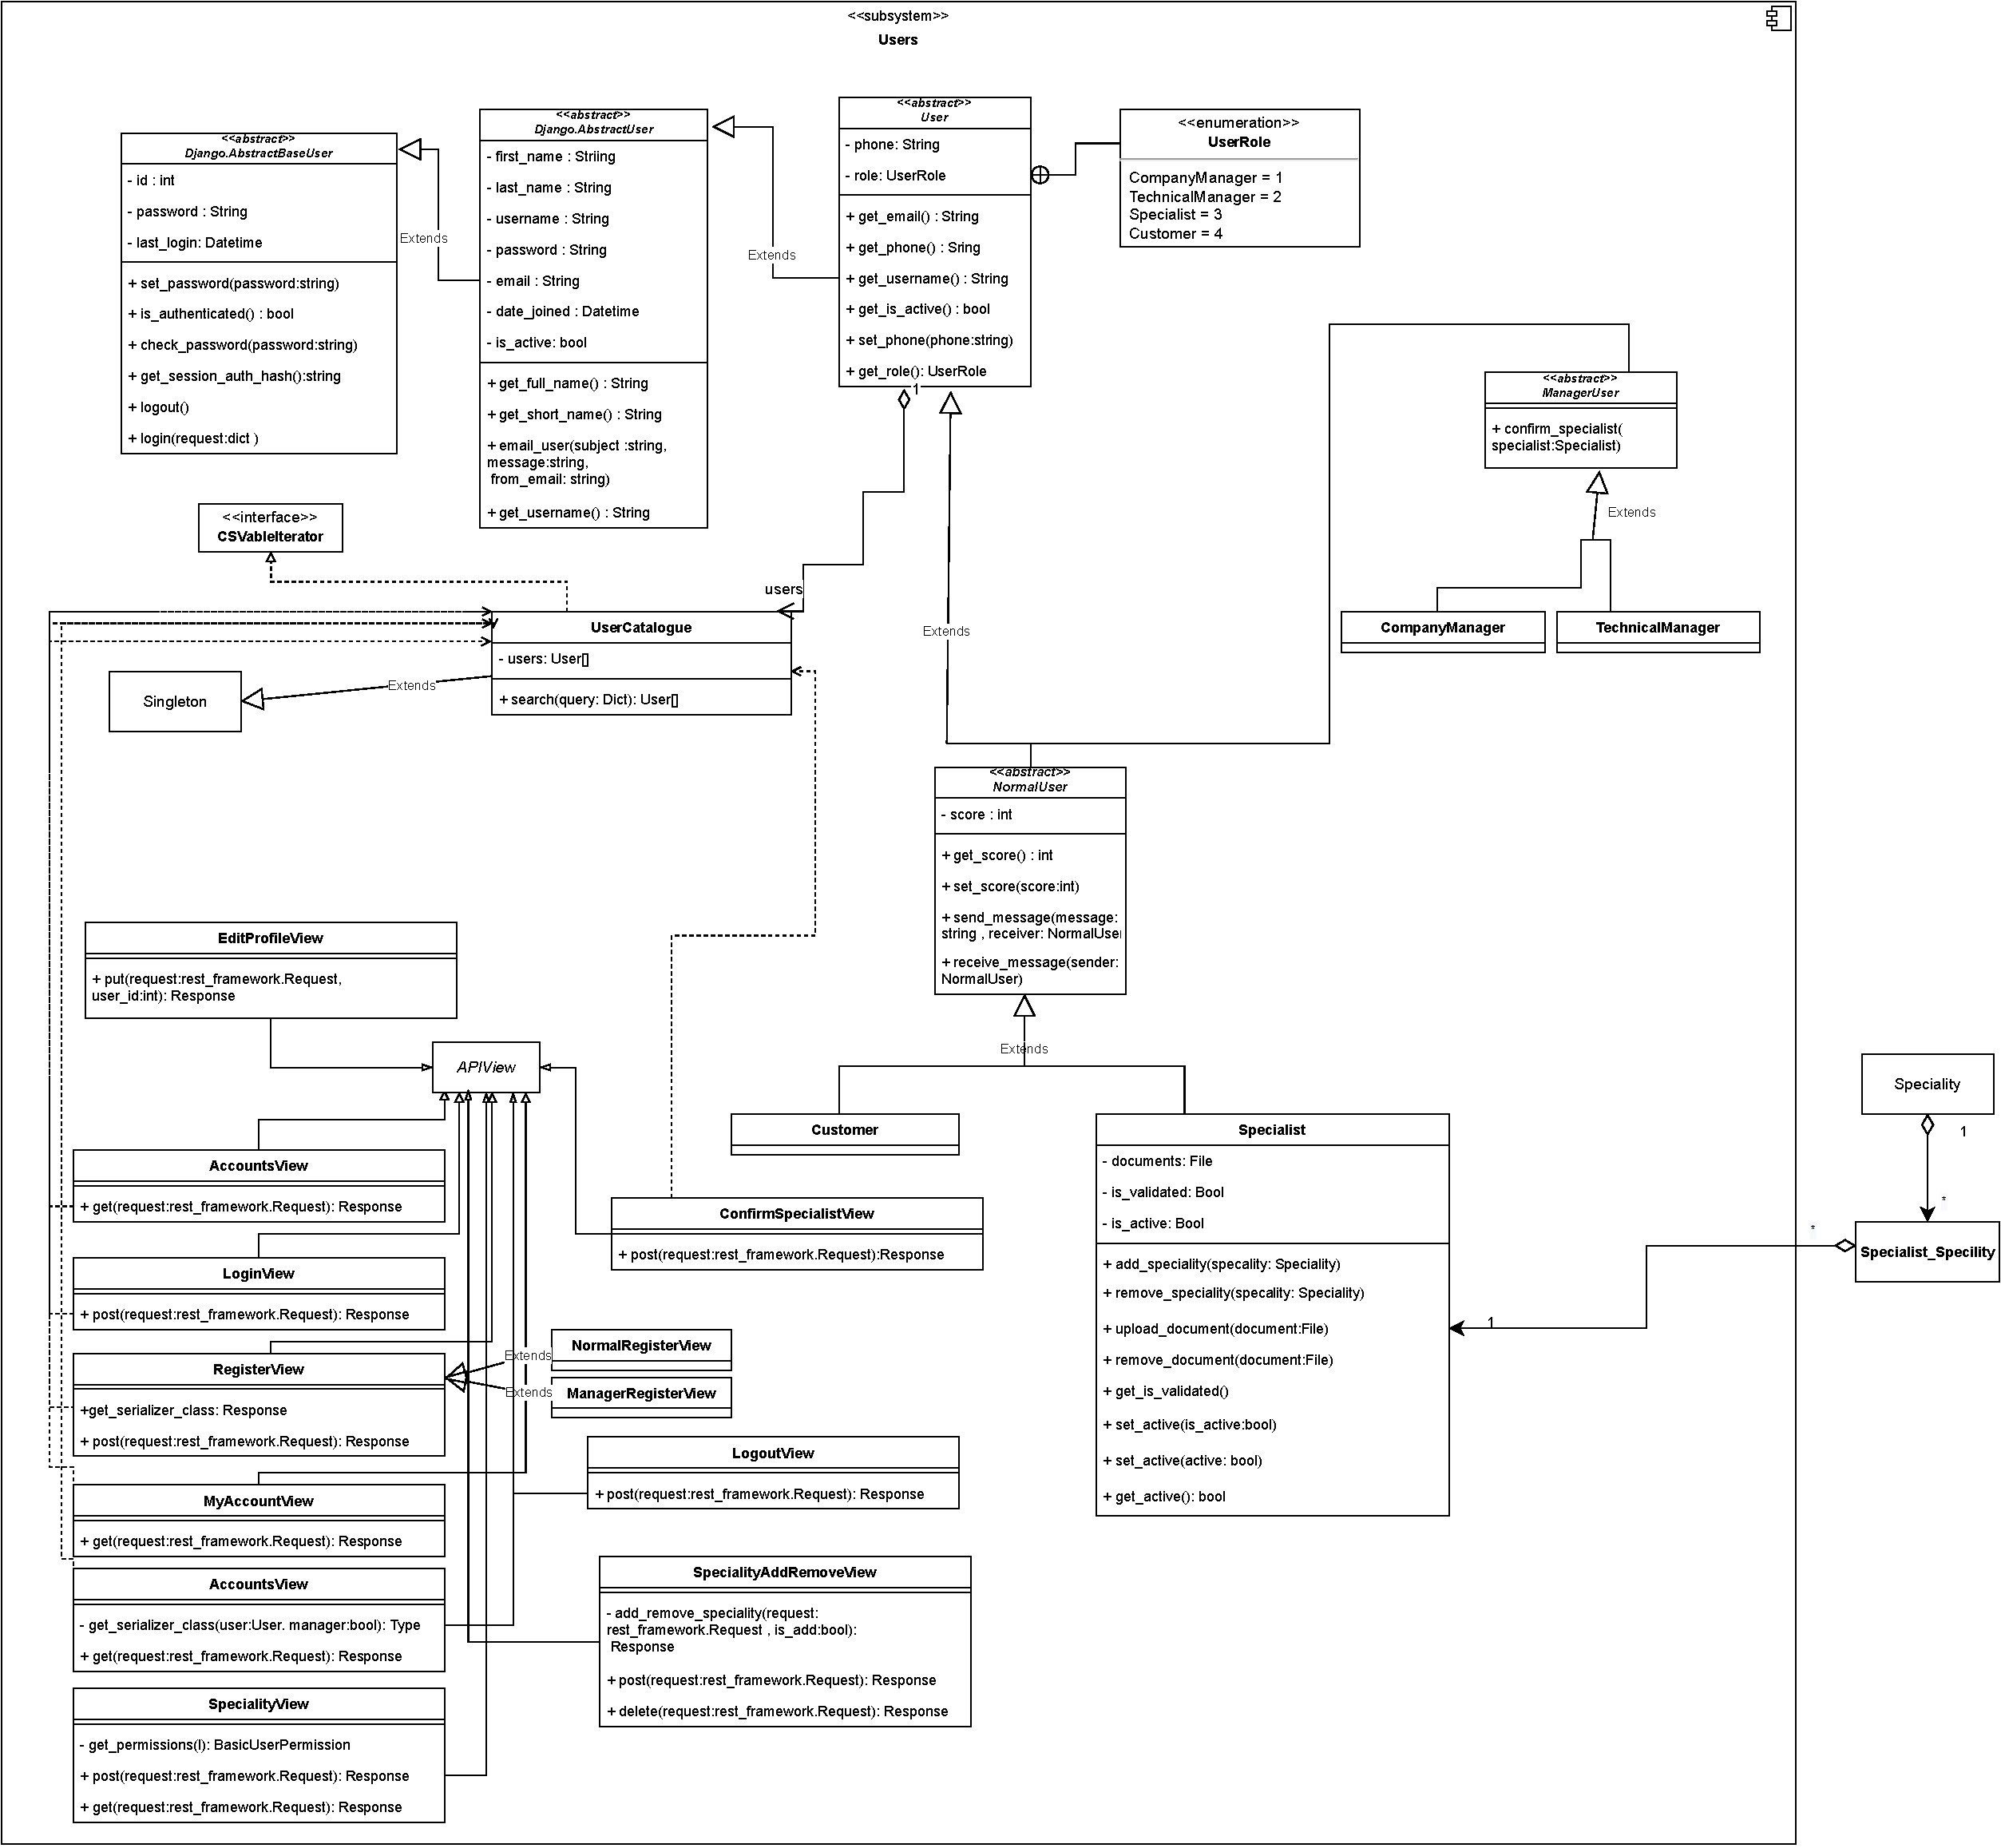
\includegraphics[scale=0.8]{figs/design-class/users.pdf}
	\caption{کلاس‌های طراحی مولفه کاربران}
\end{figure}
\FloatBarrier
\newpage


\eject \pdfpagewidth=21in \pdfpageheight=18in

\begin{figure}[ht!]
	\centering
	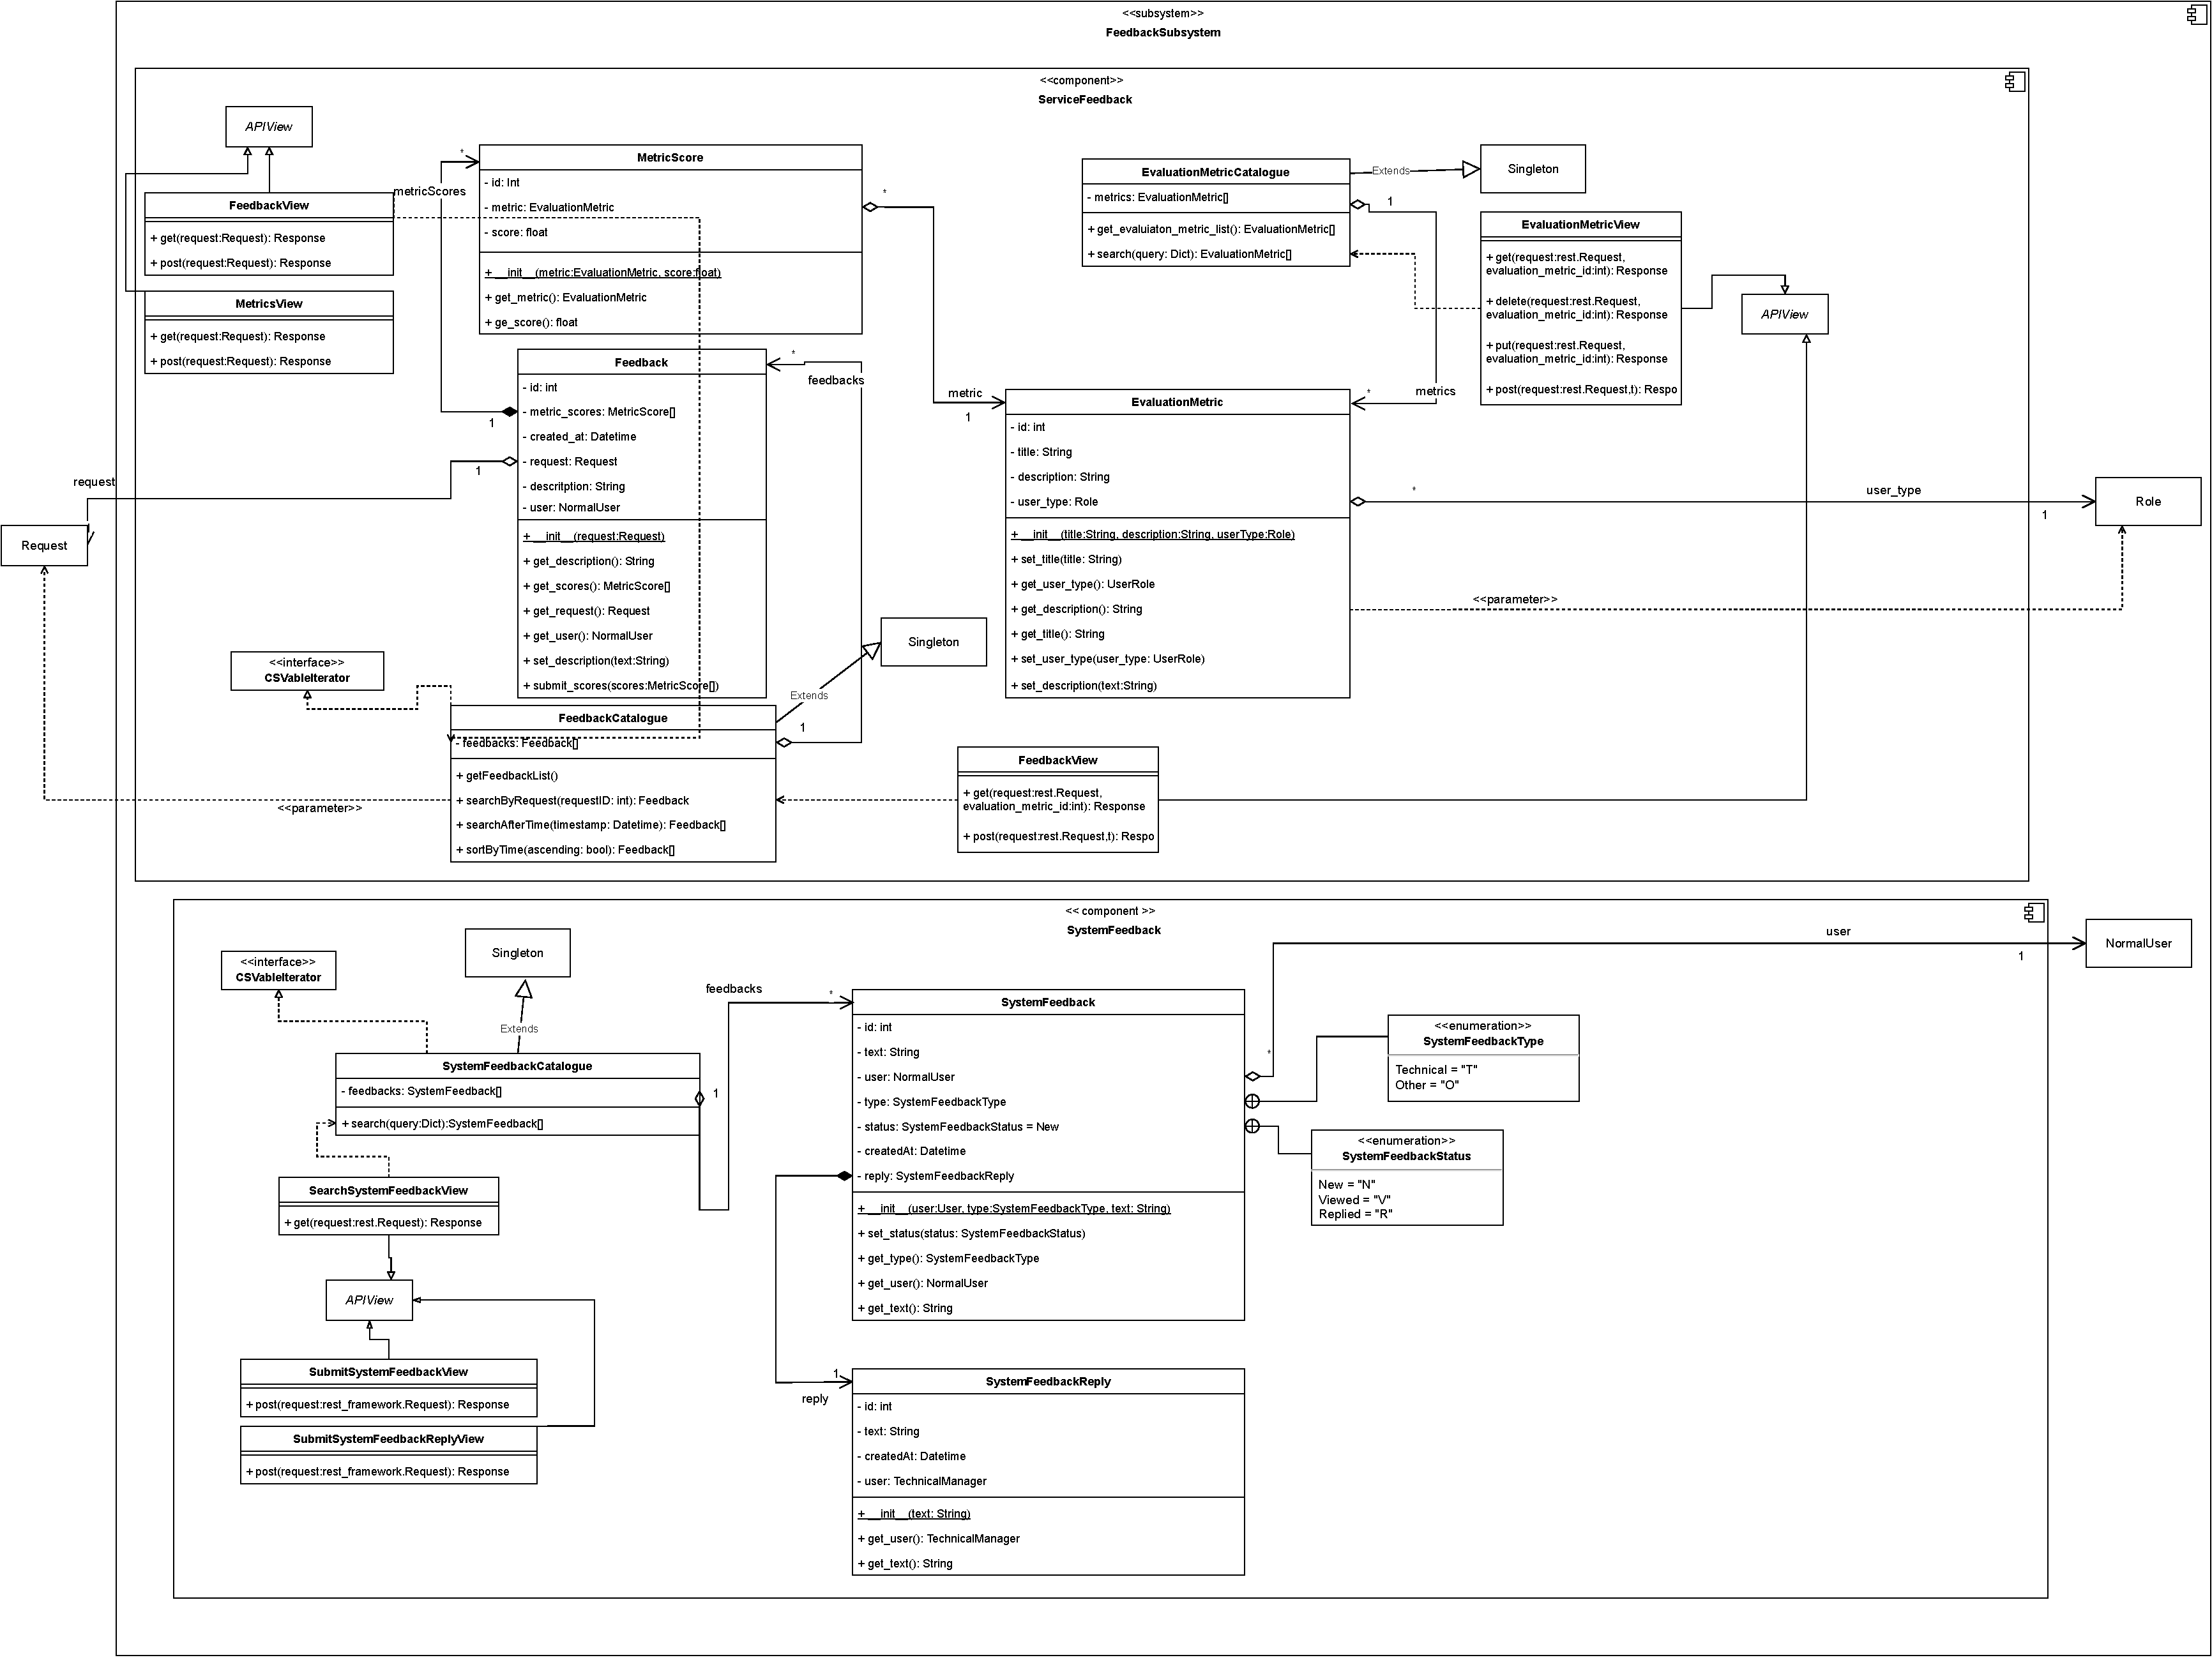
\includegraphics[scale=0.8]{figs/design-class/feedback.pdf}
	\caption{کلاس‌های طراحی مولفه بازخورد}
\end{figure}
\FloatBarrier
\newpage

\eject  \pdfpagewidth=10in \pdfpageheight=10in

\begin{figure}[ht!]
	\centering
	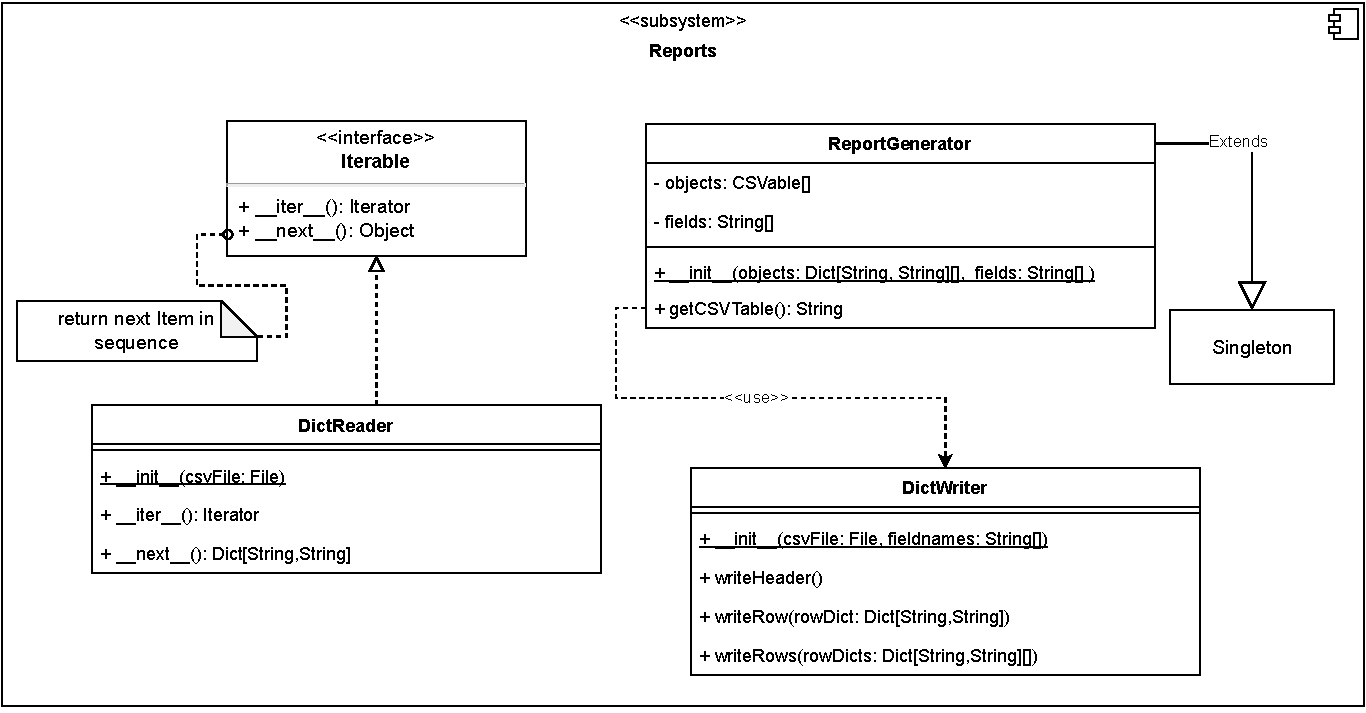
\includegraphics[scale=0.8]{figs/design-class/reports.pdf}
	\caption{کلاس‌های طراحی مولفه گزارش‌گیری}
\end{figure}
\FloatBarrier
\newpage

\KOMAoptions{paper=a4}
\recalctypearea

\begin{figure}[ht!]
	\centering
	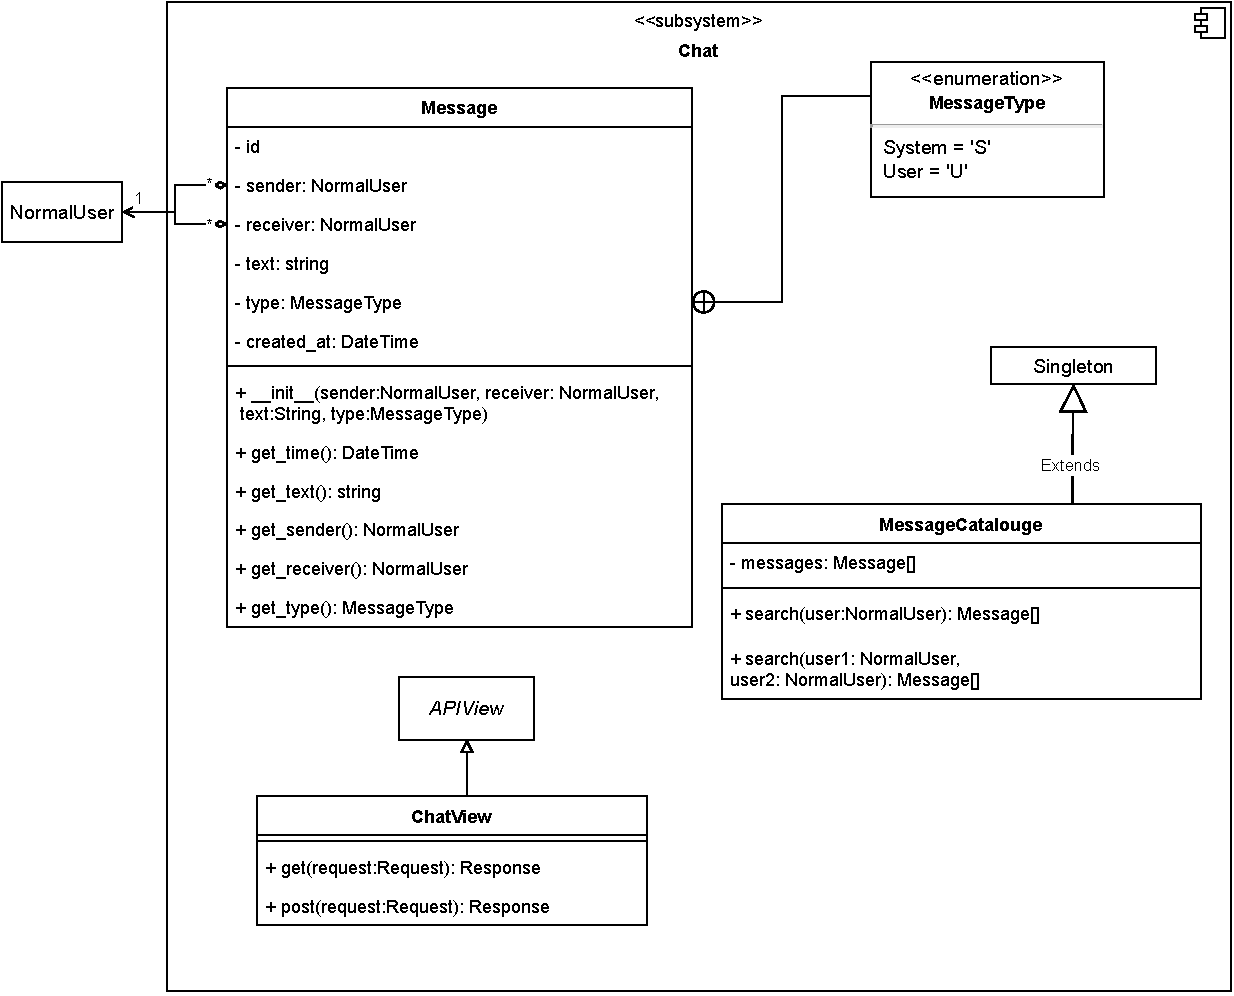
\includegraphics[scale=0.8]{figs/design-class/chat.pdf}
	\cccaption{کلاس‌های طراحی مولفه چت}
\end{figure}
\FloatBarrier
\newpage

\eject \pdfpagewidth=18in \pdfpageheight=12in

\begin{figure}[ht!]
	\centering
	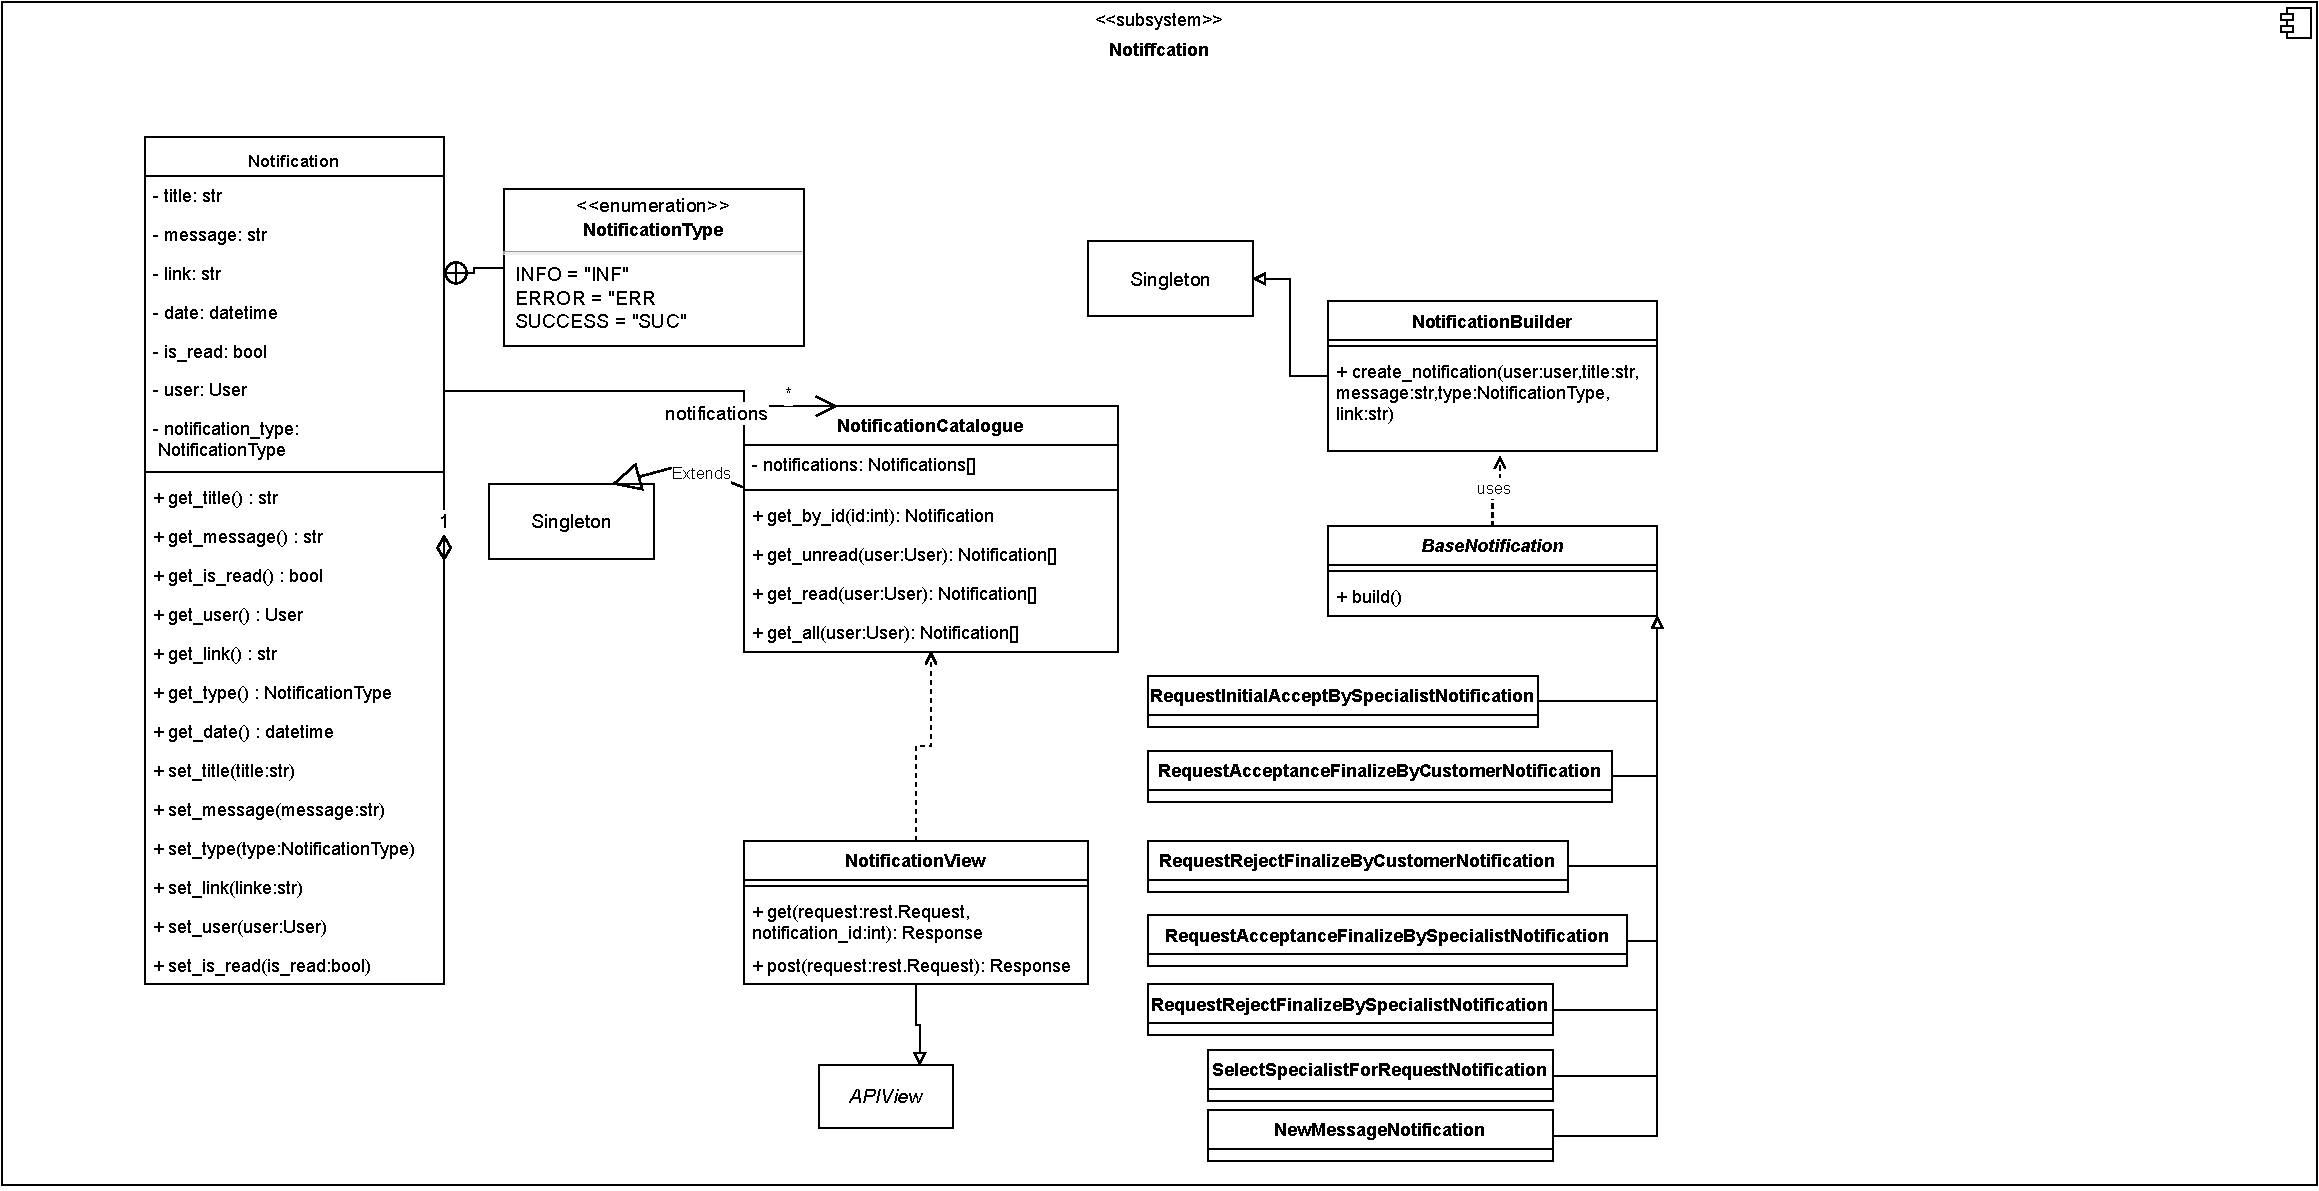
\includegraphics[scale=0.8]{figs/design-class/notification.pdf}
	\cccaption{کلاس‌های طراحی مولفه \lr{Notification}}
\end{figure}
\FloatBarrier
\newpage

\KOMAoptions{paper=a4}
\recalctypearea

\begin{figure}[ht!]
	\centering
	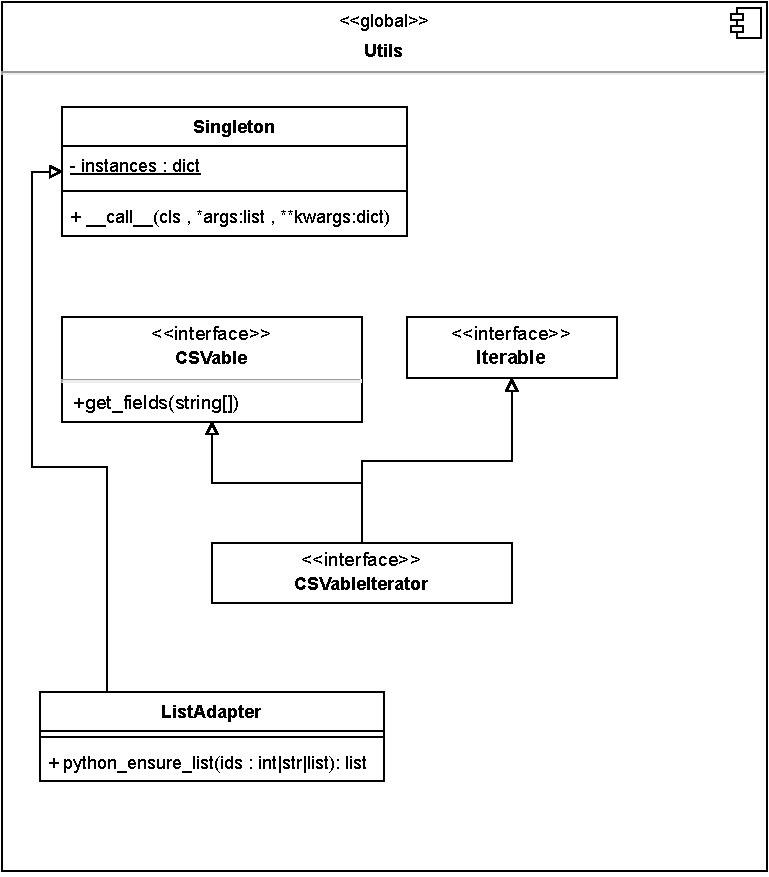
\includegraphics[scale=0.8]{figs/design-class/utils.pdf}
	\cccaption{کلاس‌های طراحی \lr{utility}}
\end{figure}
\FloatBarrier
\newpage

\eject \pdfpagewidth=16in \pdfpageheight=12in
\begin{figure}[ht!]
	\centering
	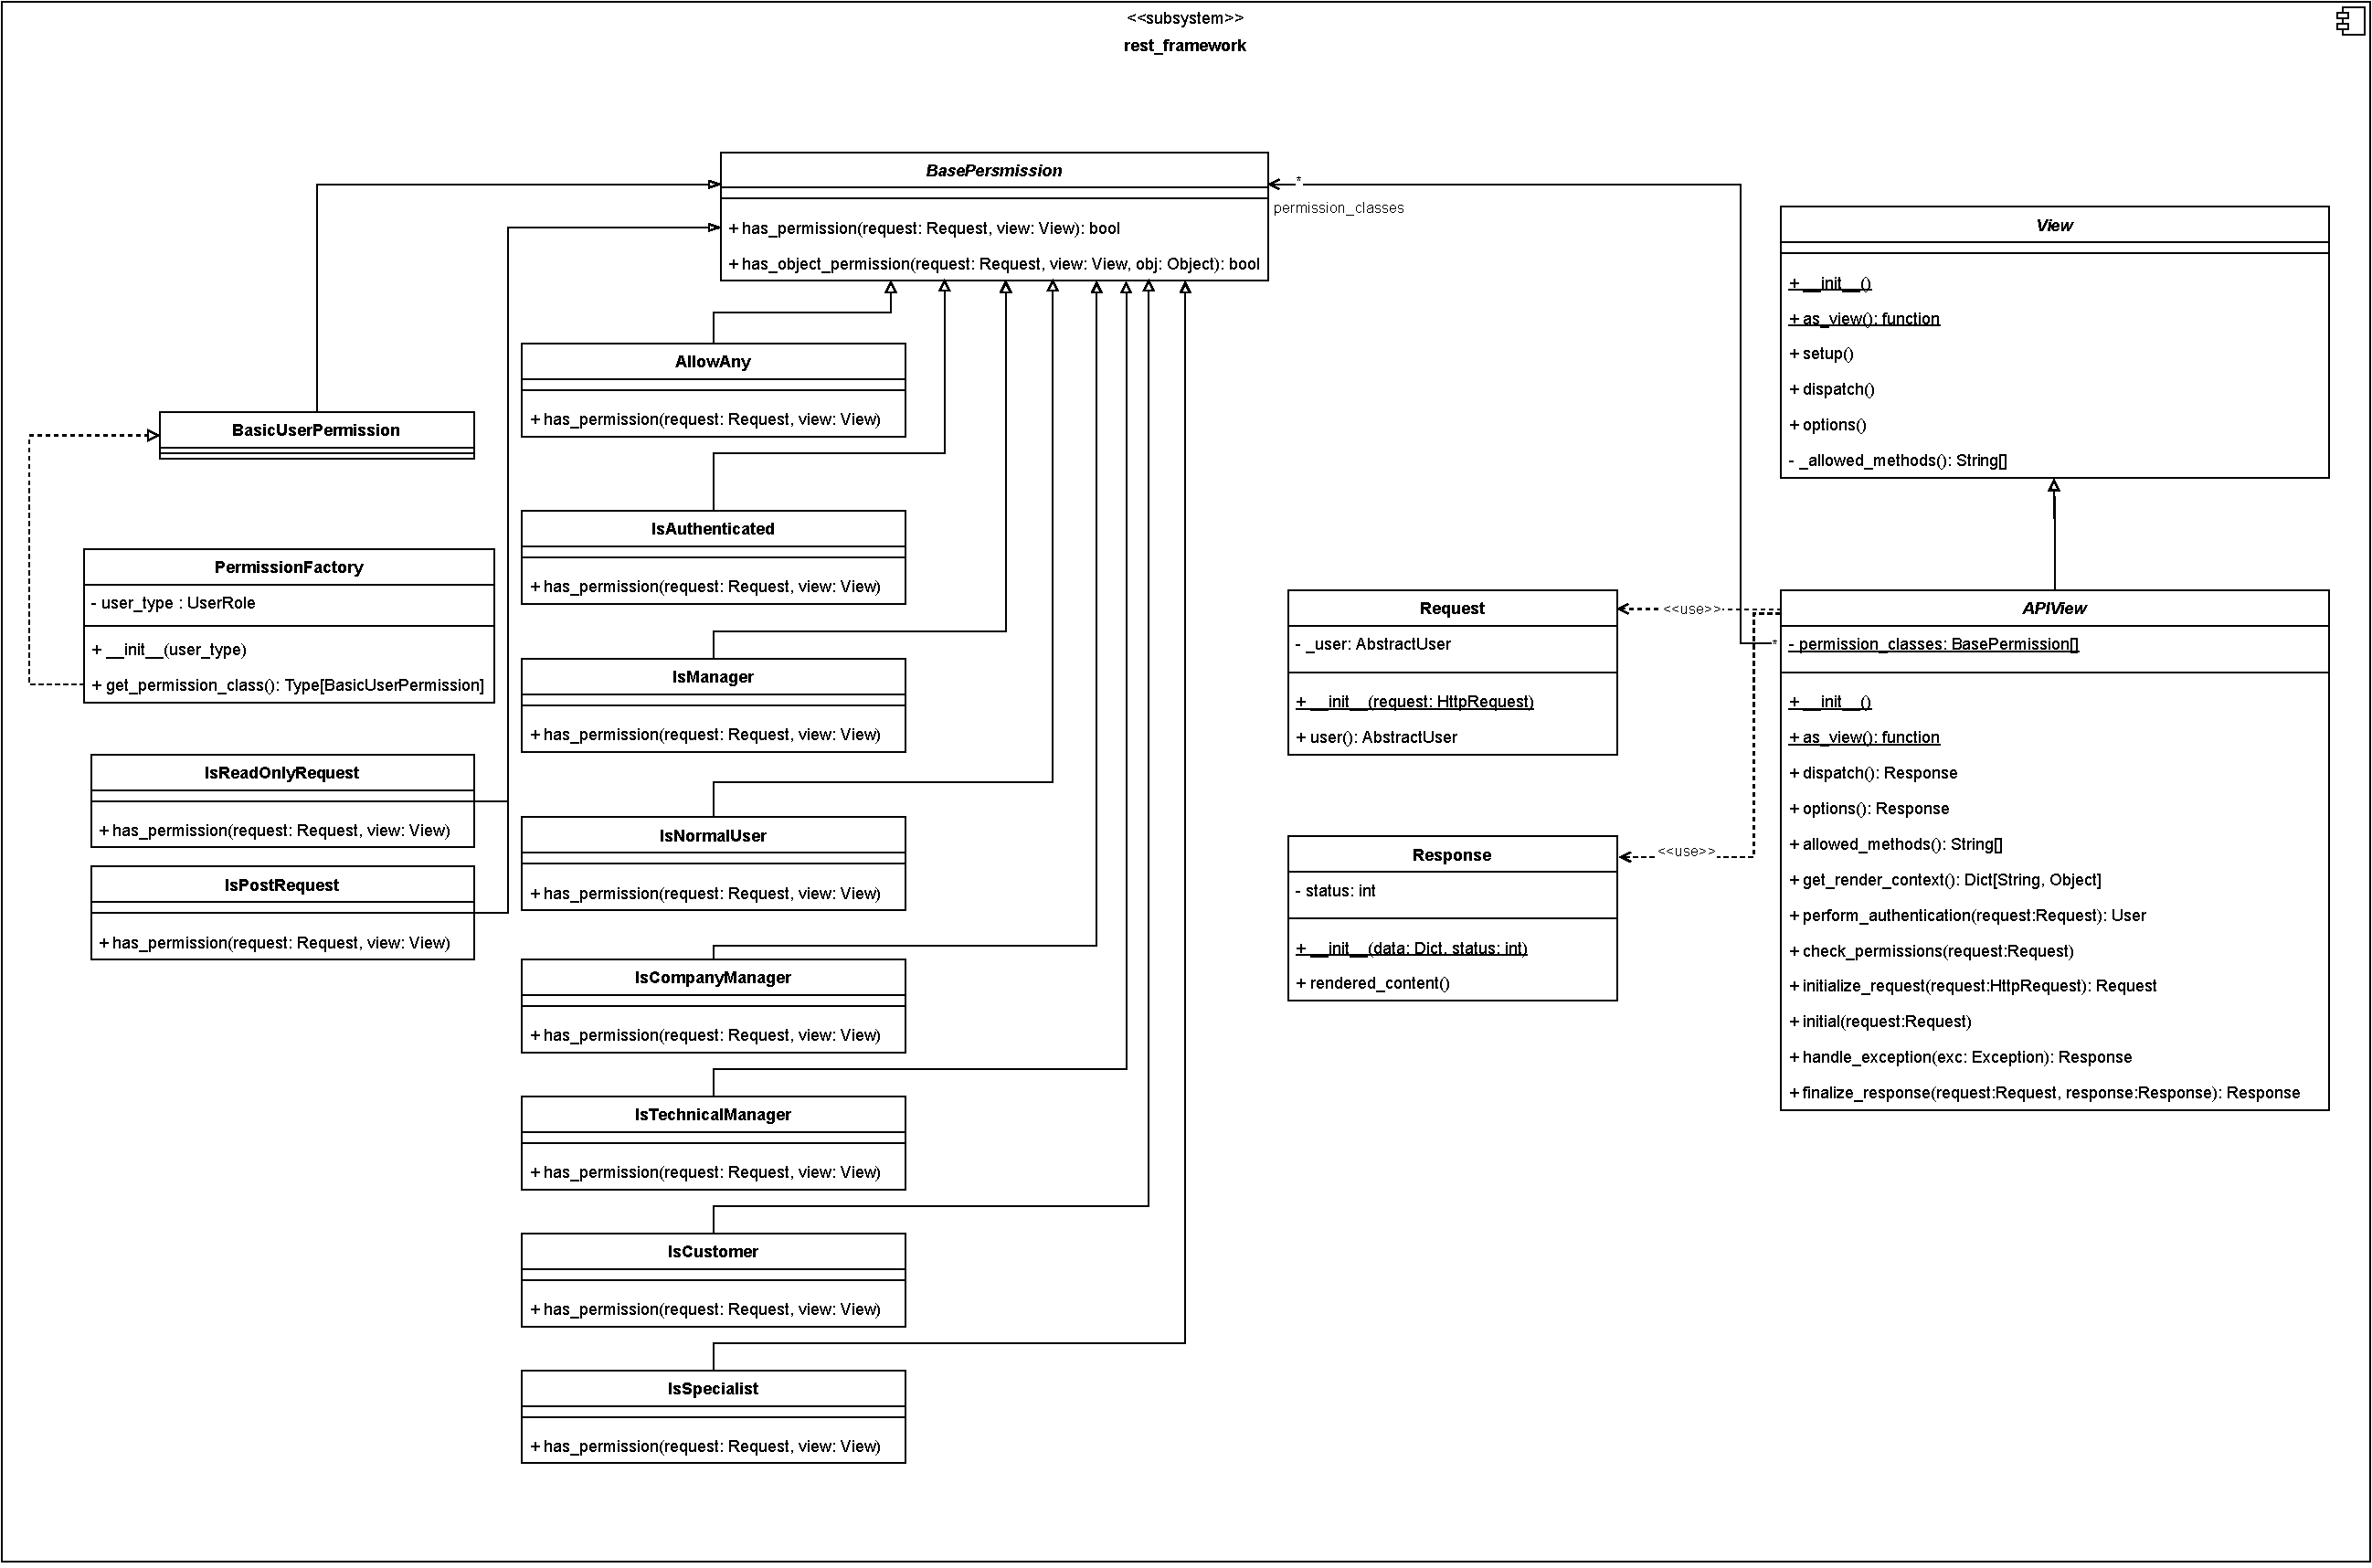
\includegraphics[scale=0.8]{figs/design-class/rest.pdf}
	\cccaption{کلاس‌های طراحی مولفه فریم‌ورک رست}
\end{figure}
\FloatBarrier
\newpage

\KOMAoptions{paper=a4}
\recalctypearea

\begin{figure}[ht!]
	\centering
	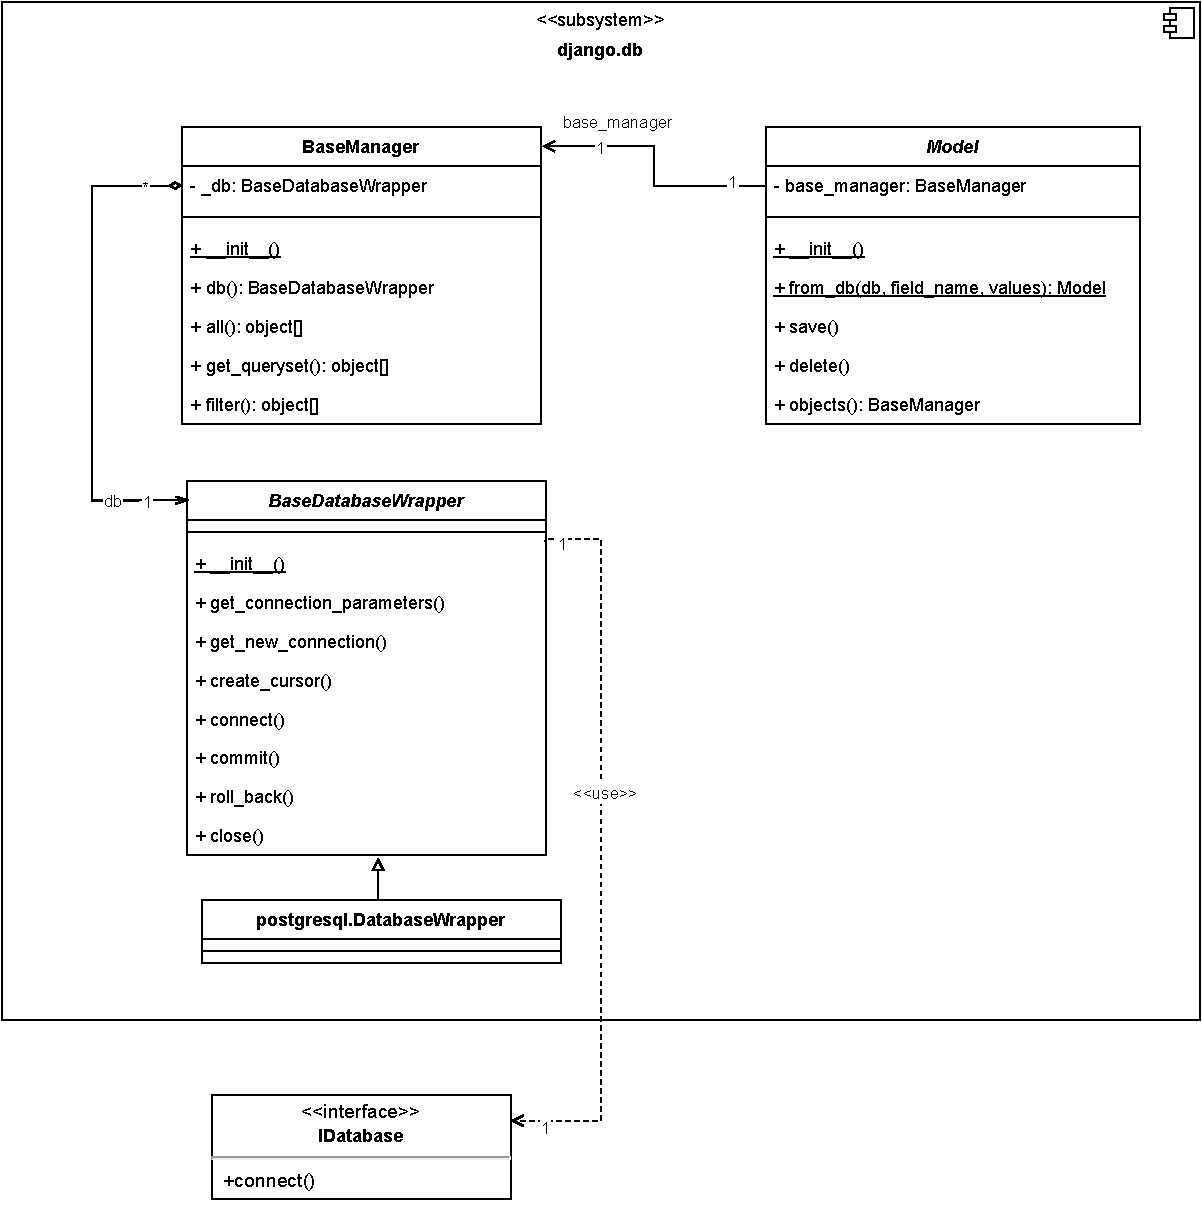
\includegraphics[scale=0.8]{figs/design-class/db.pdf}
	\cccaption{کلاس‌های طراحی مولفه دیتابیس}
\end{figure}
\FloatBarrier
\newpage

\eject \pdfpagewidth=25in \pdfpageheight=25in

\begin{figure}[ht!]
	\centering
	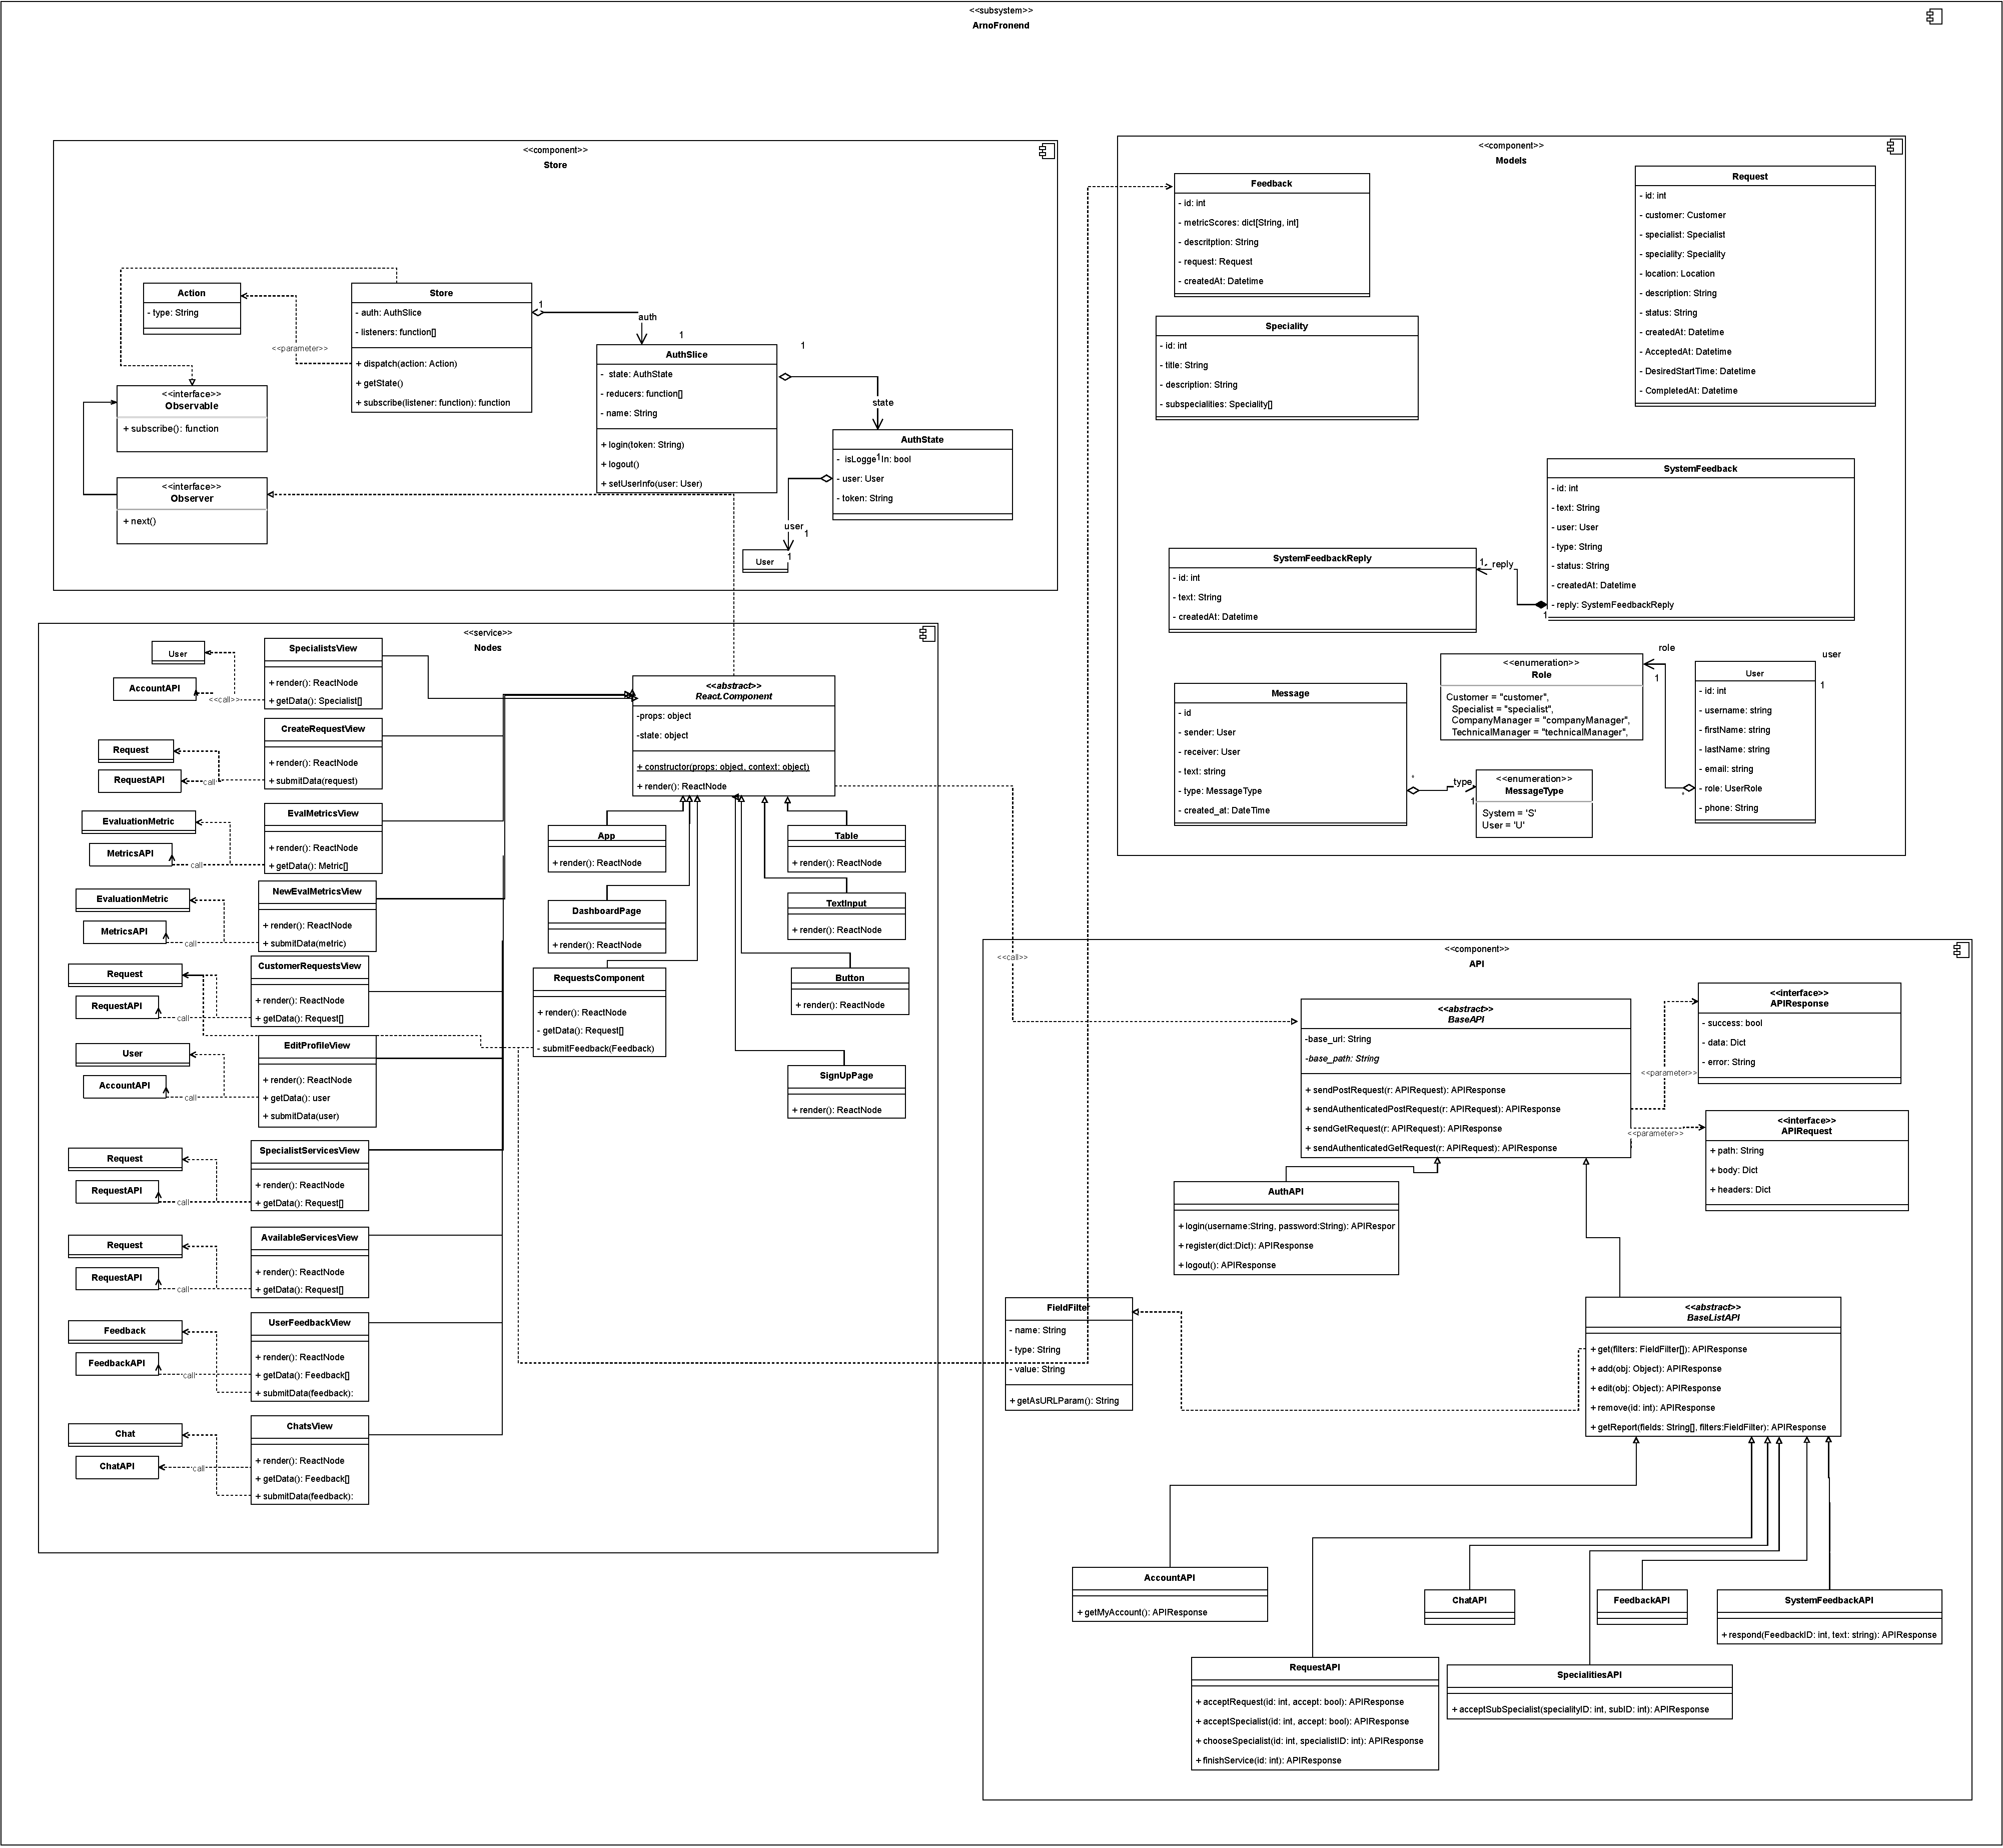
\includegraphics[scale=0.8]{figs/design-class/front.pdf}
	\cccaption{کلاس‌های طراحی رابط کاربری}
\end{figure}
\FloatBarrier
\newpage

\KOMAoptions{paper=a4}
\recalctypearea

هر کدام از این کلاس‌های سریالایزر که در ادامه آورده شده در مولفه‌های مربوط به خودشان قرار می‌گیرند و برای سریالایز کردن آبجکت‌های مختلف و تبدیل آن‌ها به JSON استفاده می‌شوند. برای پرهیز از شلوغی مولفه‌ها به طور جداگانه آورده‌شده‌اند.

هم چنین همه‌ی این کلاس‌ها از کلاس
\lr{rest\_framework.ModelSerializer}
ارث‌بری می‌کنند.

\begin{figure}[ht!]
	\centering
	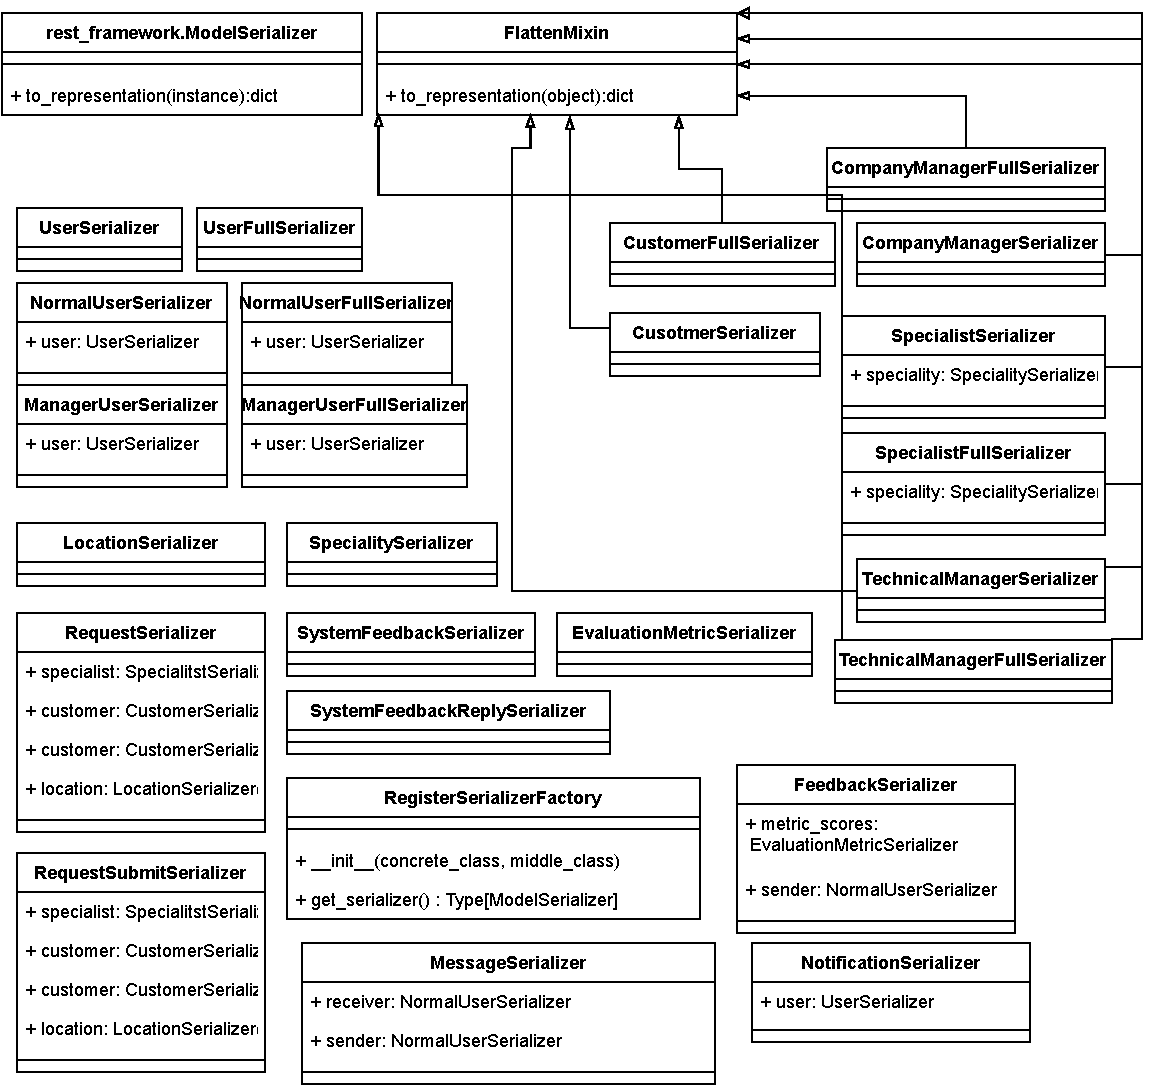
\includegraphics[scale=0.8]{figs/design-class/serial.pdf}
	\caption{کلاس‌های سریالایزر}
\end{figure}
\FloatBarrier
\newpage


\KOMAoptions{paper=a4}
\recalctypearea
\newpage

% figs/OOD-design-class-page-1.pdf